\section{Evidence from Twenty Years of Contracts and Trades}\label{sec:empirics}

\subsection{Data}

The NHL does not publish contract terms, and the most widely used public archive, CapFriendly, closed in 2024. I rebuilt the league's contract history from CapWages \citep{capwages}, which publishes, for each player, every standard player contract with its per-season cap hit and clause status (NMC, NTC, modified NTC, modified NMC), free-text clause details, and a transaction log in which every trade carries a unique identifier. I collected the pages of all 7,965 players listed in the site's index on 30 October 2026. This yielded 12,800 contracts and 27,381 contract-seasons between 2005--06 and 2026--27, together with every season already committed under signed contracts through 2034--35. Seasons are NHL league years (1 July to 30 June). Modified-clause list sizes are parsed from the clause text. Appendix~\ref{app:data} documents the variables and every coding decision.

Two checks support the data. First, coverage: matching the contract panel to official NHL season rosters, at least 94 per cent of rostered players in every season from 2014--15 onward (and 91 per cent in 2013--14) have a contract on file. Coverage falls to 75 per cent in 2009--10 and below half before 2007--08, because the archive under-represents players who retired early in the cap era. I therefore treat 2013--14 onward as the primary sample and flag earlier seasons. Second, external validity. The trade series reproduces the NHL's official count of trade-deadline-day transactions \citep{nhl_statspack} with a correlation of 0.96 and a mean absolute error of 1.1 trades per year across the 17 seasons from 2009--10 to 2025--26. The 2026--27 clause counts (306 protected contracts, 120 of them NMCs) are close to an independent August 2026 count of 312 protected players and 111 NMCs \citep{deseret_ntc}.

The trade series counts every trade that moved at least one player under contract. It does not capture pick-only trades. A ``protected trade'' is one that moved a player whose contract carried any clause in that season. Since an in-force clause must be waived for a trade to proceed, every such trade is one the player consented to.

\subsection{The rise of trade protection}

Figure~\ref{fig:prev} and Table~\ref{tab:prev} show the trend. In 2013--14, the first season of the primary sample, 158 contracts carried some form of trade protection, about five per team. By 2026--27 the number was 306, almost ten per team. Over the same period the protected share of all cap dollars rose from 31 to 49 per cent, and the protected share of star contracts (those worth at least 7.5 per cent of the cap) rose from 62 to 77 per cent. The increase was not steady. Prevalence was flat through the late 2010s and the flat-cap years, then rose sharply from 2022--23 as the cap began to grow again. The composition shifted too: NMCs, the strongest form, grew from 68 to 120.

Two features of the trend fit the model's account of protection as a non-cash currency (Proposition~\ref{prop:price}). The first is the timing of the take-off. It began as teams emerged from the flat cap carrying long commitments, and it accelerated as the 2025 CBA's shorter term limits approached. Under those conditions protection is one of the few concessions a team can offer a star without spending cap space. The second is that the protected share of new long-term deals for established players has trended up across signing cohorts (Figure~\ref{fig:cohorts}). Among multi-year contracts worth at least five per cent of the cap signed by players aged 26 or older, the share granting a full NTC or NMC at some point rose from 45--50 per cent in 2009--13 to 74 and 82 per cent in the 2024--25 and 2025--26 cohorts.

\begin{figure}[t]\centering
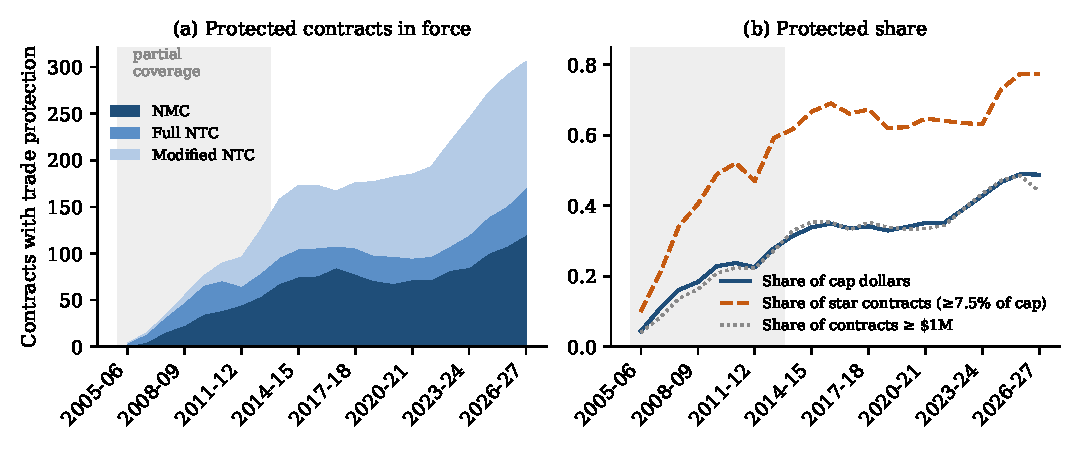
\includegraphics[width=\linewidth]{../analysis/figures/fig_prevalence.pdf}
\caption{Trade protection in force, 2005--06 to 2026--27. Shaded seasons have incomplete coverage (fewer than 90 per cent of rostered players matched to a contract). Source: author's compilation from CapWages.}\label{fig:prev}
\end{figure}

\begin{table}[t]\centering\scriptsize
\caption{Trade protection by season}\label{tab:prev}
\begin{tabular}{lrrrrrrrr}\toprule
Season & Protected & NMC & NTC & M-NTC & Per team & Share cap $ & Share stars & Median NT list\\\midrule
2009-10 & 76 & 34 & 31 & 10 & 2.5 & 0.23 & 0.49 & \\
2010-11 & 90 & 39 & 32 & 19 & 3.0 & 0.24 & 0.52 & \\
2011-12 & 96 & 45 & 20 & 31 & 3.2 & 0.23 & 0.47 & \\
2012-13 & 125 & 54 & 25 & 46 & 4.2 & 0.28 & 0.59 & 8\\
2013-14 & 158 & 68 & 28 & 62 & 5.3 & 0.31 & 0.62 & 6\\
2014-15 & 173 & 75 & 30 & 68 & 5.8 & 0.34 & 0.67 & 10\\
2015-16 & 173 & 76 & 30 & 67 & 5.8 & 0.35 & 0.69 & 10\\
2016-17 & 167 & 85 & 23 & 59 & 5.6 & 0.34 & 0.66 & 10\\
2017-18 & 176 & 78 & 28 & 70 & 5.7 & 0.34 & 0.67 & 10\\
2018-19 & 177 & 71 & 27 & 79 & 5.7 & 0.33 & 0.62 & 10\\
2019-20 & 182 & 68 & 29 & 85 & 5.9 & 0.34 & 0.62 & 10\\
2020-21 & 185 & 72 & 23 & 90 & 6.0 & 0.35 & 0.65 & 10\\
2021-22 & 193 & 72 & 25 & 96 & 6.0 & 0.35 & 0.64 & 10\\
2022-23 & 220 & 82 & 26 & 112 & 6.9 & 0.39 & 0.63 & 10\\
2023-24 & 245 & 85 & 35 & 125 & 7.7 & 0.43 & 0.63 & 10\\
2024-25 & 272 & 100 & 39 & 133 & 8.5 & 0.47 & 0.73 & 10\\
2025-26 & 291 & 107 & 43 & 140 & 9.1 & 0.49 & 0.77 & 10\\
2026-27 & 306 & 119 & 51 & 135 & 9.6 & 0.49 & 0.77 & 10\\
\bottomrule\end{tabular}
\begin{minipage}{0.95\linewidth}\footnotesize\vspace{4pt}
\emph{Notes:} Counts of contracts in force with each clause type in each league year. ``Share cap \$'' is the protected share of all cap hits on file. ``Share stars'' is the protected share among contracts worth at least 7.5 per cent of the upper limit. ``Median NT list'' is the median number of teams on parsed modified no-trade lists. Seasons before 2013--14 have incomplete coverage.
\end{minipage}
\end{table}

\paragraph{The protection overhang.} The forward view is more striking still (Table~\ref{tab:forward}, Figure~\ref{fig:forward}). On contracts already signed as of 30 October 2026, \$1.65 billion of 2027--28 cap hits belongs to players with trade protection. That is 45 per cent of the league-wide ceiling implied by the projected \$113.5 million cap. Because protected deals are the long ones, protected players also account for a rising share of whatever is committed further out: 67 per cent of committed dollars in 2028--29 and 80 per cent in 2030--31. Part of this share is mechanical, because short unprotected deals have not yet been signed for those seasons. The levels are not mechanical: 220 protected contracts are already in force for 2028--29. Whatever the next CBA does, the clauses Bettman criticised will shape the trade market for the rest of the decade.

\begin{figure}[t]\centering
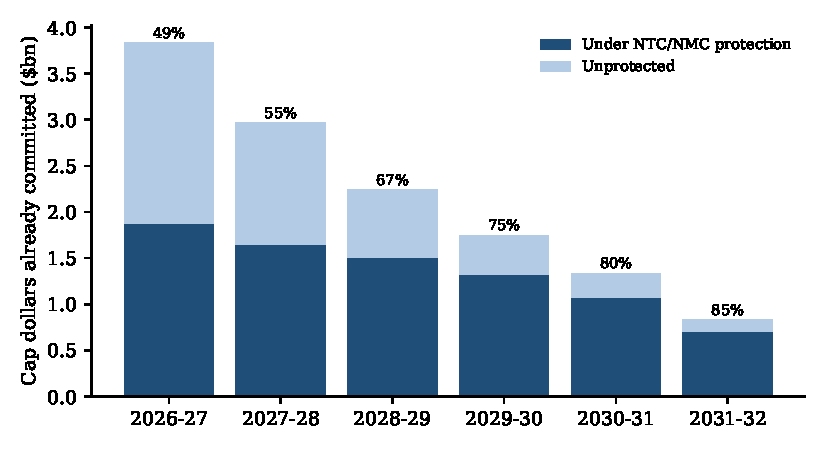
\includegraphics[width=0.75\linewidth]{../analysis/figures/fig_forward.pdf}
\caption{Cap dollars already committed for future seasons as of 30 October 2026, by protection status. Labels give the protected share of committed dollars.}\label{fig:forward}
\end{figure}

\begin{table}[t]\centering\small
\caption{The protection overhang: commitments already signed as of 30 October 2026}\label{tab:forward}
\begin{tabular}{lrrrrrr}\toprule
Season & Protected & NMC & Full NTC/NMC & Protected \$M & All committed \$M & Protected share\\\midrule
2026-27 & 306 & 120 & 170 & 1,871 & 3,834 & 0.49\\
2027-28 & 250 & 97 & 124 & 1,646 & 2,972 & 0.55\\
2028-29 & 220 & 73 & 91 & 1,504 & 2,242 & 0.67\\
2029-30 & 182 & 52 & 64 & 1,320 & 1,750 & 0.75\\
2030-31 & 138 & 36 & 38 & 1,072 & 1,338 & 0.80\\
2031-32 & 82 & 23 & 22 & 707 & 831 & 0.85\\
\bottomrule\end{tabular}
\end{table}

\subsection{Protection and the trade market}

\paragraph{Season-level patterns.} Across the 17 complete league years from 2009--10 to 2025--26, the protected share of cap dollars is positively correlated with total trade volume ($r=0.50$). That correlation disappears once the controls in Table~\ref{tab:season} are added: cap growth, the flat-cap years, shortened seasons, expansion-draft years and a linear trend. With 17 observations and trending series, the honest summary is that rising protection has not visibly reduced the overall volume of trades or of star trades. What it has changed is the \emph{composition} of trades. The share of trades that move a protected player tracks prevalence closely ($r=0.91$). It rose from roughly one in six in the 2010s to 30 per cent in 2024--25 and 26 per cent in 2025--26, and the relationship survives the controls (coefficient 1.34, $p<0.01$). A growing fraction of the league's transactions therefore pass through a player veto. Contemporary accounts of the quiet 2026 deadline say the same: vetoes, alongside new cap rules, kept several large deals from happening \citep{tsn_deadline2026}.

\begin{figure}[t]\centering
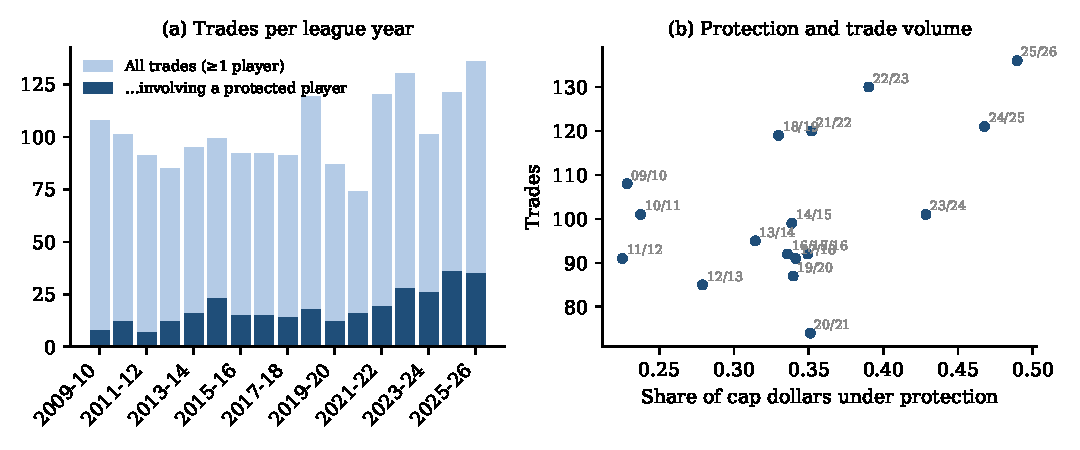
\includegraphics[width=\linewidth]{../analysis/figures/fig_trades.pdf}
\caption{Trades by league year and the share involving a protected player (a), and the protected share of cap dollars against trade volume (b), 2009--10 to 2025--26.}\label{fig:trades}
\end{figure}

\begin{table}[t]\centering\small
\caption{Season-level regressions, 2009--10 to 2025--26}\label{tab:season}
\begin{tabular}{lcccc}\toprule
 & All trades & Star trades & Deadline-day & Share w/ protected\\\midrule
Protected share of cap \$ & -40.14 & 42.45 & -40.95 & 1.34$^{*}$\\
 & (173.80) & (34.24) & (91.33) & (0.45)\\
Cap growth (pct.) & 71.80 & -11.12 & -31.41 & 0.05\\
 & (82.21) & (17.44) & (61.34) & (0.18)\\
Flat-cap era & 13.75 & 7.21 & -3.48 & 0.04\\
 & (10.20) & (3.75) & (8.20) & (0.03)\\
Shortened season & -27.05$^{*}$ & -5.53 & 0.12 & 0.01\\
 & (10.08) & (2.94) & (6.19) & (0.03)\\
Expansion draft year & -15.99$^{*}$ & -3.54 & -2.03 & -0.01\\
 & (5.09) & (2.06) & (4.30) & (0.01)\\
Linear trend & 2.07 & -0.70 & 1.00 & -0.01\\
 & (2.54) & (0.60) & (1.48) & (0.01)\\
Constant & 103.40$^{*}$ & -0.08 & 29.52 & -0.21$^{*}$\\
 & (43.55) & (7.46) & (21.44) & (0.10)\\
N & 17 & 17 & 17 & 17\\
$R^2$ & 0.75 & 0.80 & 0.21 & 0.88\\
\bottomrule\end{tabular}
\begin{minipage}{0.95\linewidth}\footnotesize\vspace{4pt}
\emph{Notes:} OLS with HC3 standard errors in parentheses; $^{*}p<0.05$. ``Star trades'' move at least one player whose cap hit is at least 7.5 per cent of the upper limit. ``Deadline-day'' trades are those on the busiest February--April date of each season, which coincides with the official deadline in every season checked. Shortened seasons: 2012--13, 2019--20, 2020--21. Expansion-draft years: the seasons on either side of the 2017 and 2021 expansion drafts.
\end{minipage}
\end{table}

\paragraph{Player-level trade hazards.} The cleaner test uses the player-season panel. Table~\ref{tab:hazard} estimates the probability that a player is traded in a given season, for players aged 26 or older earning at least three per cent of the cap, from 2013--14 to 2025--26. The controls are cap share, age, years remaining, position, prior-season scoring and season fixed effects. Unconditionally, 19.5 per cent of unprotected player-seasons in this group end in a trade, against 10.7 per cent of protected ones. Conditionally, a full NTC lowers the annual trade probability by about 7 percentage points and an NMC by about 8, against a mean of 14 per cent. These are reductions of roughly half. A modified NTC lowers it by only 3 points ($p\approx0.05$--$0.10$). Among stars, the NMC effect is the same size and is half of a smaller base rate. Clauses therefore do what they say: they keep players in place. But the protected players who \emph{are} traded are, by construction, traded on terms they accept. That is the condition under which the model predicts the seller's return collapses.

\begin{table}[t]\centering\small
\caption{Probability of being traded in a season, by clause type (2013--14 to 2025--26)}\label{tab:hazard}
\begin{tabular}{lcccc}\toprule
 & (1) LPM & (2) LPM & (3) LPM, stars & (4) Logit\\\midrule
Modified NTC & -0.030 & -0.026 & -0.050 & -0.173\\
 & (0.016) & (0.016) & (0.034) & (0.120)\\
Full NTC & -0.071$^{*}$ & -0.073$^{*}$ & -0.025 & -0.645$^{*}$\\
 & (0.019) & (0.019) & (0.042) & (0.224)\\
NMC & -0.081$^{*}$ & -0.082$^{*}$ & -0.082$^{*}$ & -0.855$^{*}$\\
 & (0.016) & (0.016) & (0.028) & (0.181)\\
Cap hit (share of cap) & 0.480 & 0.682 & 0.528 & 16.060\\
 & (1.081) & (1.105) & (4.333) & (12.272)\\
Points per game, prior season &  & -0.060$^{*}$ & -0.050 & -0.545$^{*}$\\
 &  & (0.025) & (0.033) & (0.244)\\
N (player-seasons) & 3947 & 3791 & 1049 & 3791\\
Mean of DV & 0.141 & 0.142 & 0.071 & 0.142\\
\bottomrule\end{tabular}
\begin{minipage}{0.95\linewidth}\footnotesize\vspace{4pt}
\emph{Notes:} Player-seasons for players aged 26 or older at the start of the season with a cap hit of at least 3 per cent of the upper limit. The omitted category is no clause. All models include age and its square, cap share squared, years-remaining indicators, a goaltender indicator and season fixed effects. Standard errors are clustered by player; $^{*}p<0.05$. Column (3) restricts to cap hits of at least 7.5 per cent. Column (4) reports logit coefficients.
\end{minipage}
\end{table}

\subsection{Is protection priced?}

Proposition~\ref{prop:price} predicts that a clause should be paid for with a lower wage, by an amount that rises with the perceived probability of a demand. Table~\ref{tab:hedonic} tests this on 496 new multi-year skater contracts signed by players aged about 26 or older, from 2009--10 to 2026--27. The dependent variable is the log of the first-season cap share. Controls are platform-season points per game (with a separate slope for defencemen), games played, age, log term and signing-year fixed effects. Protected contracts carry cap shares about 9 per cent \emph{higher}, not lower. Splitting by type, the premium sits entirely with full NTCs and NMCs. There is no sign that contracts signed in 2026--27 price protection differently, although that cohort is small.

The premium does not mean the clause is literally worth money to the team. Clauses go to players with bargaining power that the controls only partly capture, so the coefficient is an upper bound on any true compensating differential. A causal estimate would need an instrument, and the most promising candidate is the Article 11.8 eligibility threshold. The point is negative: there is no evidence of the discount the efficient-pricing benchmark requires. This contrasts with \citet{pedacehall2012} for baseball. Whether because general managers have underestimated $q$, or because the cap makes protection the cheapest currency available, teams have been granting vetoes without visibly charging for them. The 2026 wave is the event that should reprice them. Section~\ref{sec:implications} describes what repricing would look like.

\begin{table}[t]\centering\small
\caption{The price of protection: log first-season cap share on new skater contracts}\label{tab:hedonic}
\begin{tabular}{lccc}\toprule
 & (1) & (2) & (3)\\\midrule
Any protection & 0.086$^{*}$ & 0.027 & 0.086$^{*}$\\
 & (0.020) & (0.024) & (0.020)\\
Full NTC/NMC (vs. modified) &  & 0.097$^{*}$ & \\
 &  & (0.021) & \\
Any protection $\times$ signed 2026-27 &  &  & 0.008\\
 &  &  & (0.043)\\
Points/game, platform season & 0.558$^{*}$ & 0.540$^{*}$ & 0.558$^{*}$\\
 & (0.034) & (0.033) & (0.034)\\
log(term in seasons) & 0.304$^{*}$ & 0.268$^{*}$ & 0.304$^{*}$\\
 & (0.028) & (0.029) & (0.028)\\
Age at signing & -0.121 & -0.135$^{*}$ & -0.121\\
 & (0.064) & (0.063) & (0.064)\\
N (contracts) & 496 & 496 & 496\\
$R^2$ & 0.60 & 0.62 & 0.60\\
\bottomrule\end{tabular}
\begin{minipage}{0.95\linewidth}\footnotesize\vspace{4pt}
\emph{Notes:} New contracts with term of at least three seasons and a cap hit of at least 5 per cent of the upper limit, signed by players aged at least 25.5, 2009--10 to 2026--27; skaters with more than 20 platform-season games. All models include age squared, a defence indicator, its interaction with points per game, platform games played and signing-year fixed effects. HC3 standard errors; $^{*}p<0.05$. ``Any protection'' means any clause in any season of the contract.
\end{minipage}
\end{table}

\begin{figure}[t]\centering
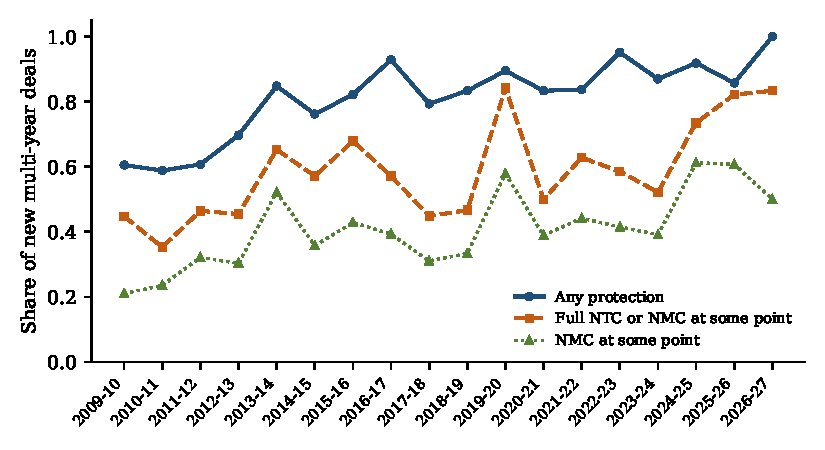
\includegraphics[width=0.75\linewidth]{../analysis/figures/fig_cohorts.pdf}
\caption{Protection in new multi-year contracts for established players, by signing year (term $\geq3$, cap hit $\geq5\%$, age $\geq25.5$). The 2026--27 cohort is partial (signings to 30 October 2026).}\label{fig:cohorts}
\end{figure}

\subsection{The case dataset}

To study what happens once a protected player wants out, I coded 25 cases between 2007--08 and 2026--27 (Appendix Table~\ref{tab:cases}). There are 16 player-initiated or mutual exits by protected players (including the ambiguous Luongo request and the disputed Kessel request), four exits by stars without a clause (Duchene, Dubois, Eichel and Hughes), and five protected stars who used their clause to stay, to choose a destination, or to veto a team-initiated deal without demanding out (Sundin, Marner, Iginla, Kane, and Werenski's reported veto). Each case records the request date and whether it was formal, informal, private or public, the clause, the number of approved destinations where reported, vetoes, days to resolution, and the return. The return is measured in two ways. The first is \emph{pick capital}, the sum of incoming draft picks valued with an empirical chart of expected career games by draft slot built from the 2005--14 drafts and normalised to the 16th pick (Appendix Figure~\ref{fig:pickvalue}). The second is \emph{realised games}, the NHL games that incoming players played in the three seasons after the trade, computed only for trades completed by 2023--24. Both measures are crude, and with this few cases they are best read as structured description.

The comparisons nonetheless line up with the model (Figure~\ref{fig:cases}). Protected demands returned less than unprotected ones on both measures: 0.84 against 1.27 mid-first-round equivalents in picks, and 263 against 354 realised games. They did not resolve faster (142 days against 170), which is consistent with clauses lowering the cost of waiting. Demands that were public from the start returned 0.44 mid-first equivalents in picks, against 1.48 for those that began privately, as Proposition~\ref{prop:audience} predicts. They also resolved faster (120 against 178 days), which is the point of going public. The realised-games measure points the other way, however: 309 games for public-from-the-start demands against 256 for those that began privately. The audience-cost result therefore rests on draft capital alone and should be treated as suggestive. Among protected cases with a reported list, the number of approved destinations is positively rank-correlated with realised games ($\rho=0.63$, $n=8$, $p=0.10$) but not with pick capital. Tkachuk's three first-round picks from a four-team list are the conspicuous outlier, discussed below.

\begin{figure}[t]\centering
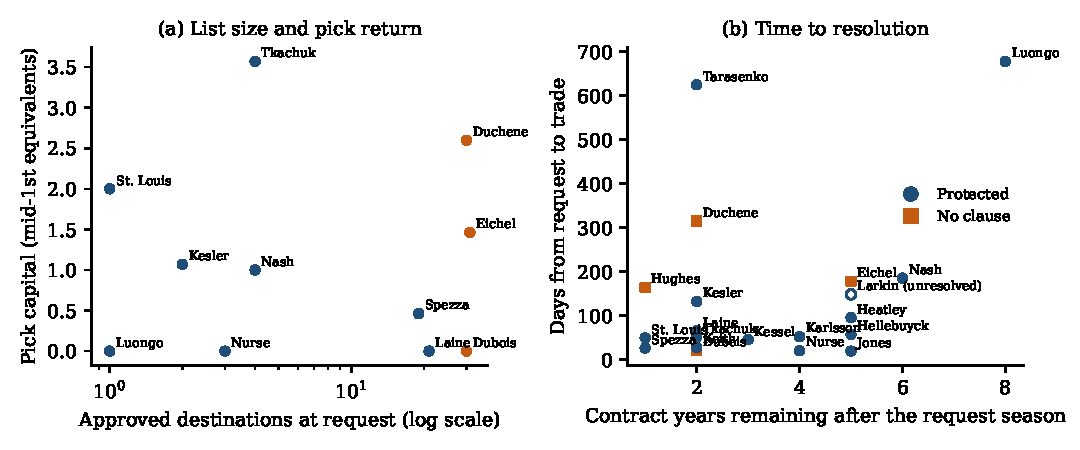
\includegraphics[width=\linewidth]{../analysis/figures/fig_cases.pdf}
\caption{Approved destinations and pick return (a), and contract years remaining and days to resolution (b), for trade demands 2009--2026. Larkin's request is unresolved (censored at 30 October 2026).}\label{fig:cases}
\end{figure}
